%\clearpage
\section{Chromosome-shaped oxidation of MoRe thin films}
\label{sec:more}

The use of MoRe as superconductor of choice for our devices has a rather anectodal reason:
%
In 2012, Schneider \textit{et al.}~\cite{schneiderCouplingCarbonNanotube2012,schneiderSuspendedCarbonNanotubes2014b} were searching for a superconductor able to withstand high magnetic fields as well as the growth conditions for carbon nanotube (CNT) fabrication, with good superconducting contacts.
%
Initial attempts with NbTiN, then the superconductor of choice in the neighboring groups of Teun Klapwijk~\cite{iosadSourceOptimizationMagnetron1999} and Leo Kouwenhoven~\cite{mourikSignaturesMajoranaFermions2012}, showed poor performance under CNT growth conditions, low CNT yield and high contact resistance.
%
Rhenium, also previously used in the group of Leo Kouwenhoven~\cite{keijzersJosephsonEffectsCarbon2012}, performed significantly better, but a material with even higher $T_\text{c}$ was found in the form of molybdenum rhenium (MoRe):
%
MoRe turned out to survive the CNT growth, have a very closely matching work function to the one of CNTs, and yield larger $T_\text{c}$ and $I_\text{c}$ compared to rhenium.

MoRe was since the superconductor of choice for CNTs.
%
Soon after, it was picked up by other groups, not only in the field of graphene~\cite{azizMolybdenumrheniumSuperconductingSuspended2014a}, most notably after Calado \textit{et al.} were able to show ballistic superconductivity in edge-contacted graphene~\cite{caladoBallisticJosephsonJunctions2015d}, and has since been used in numerous groups with notable success, see Refs.~\cite{singhMolybdenumrheniumAlloyBased2014,gotzCosputteredMoReThin2016,blienCarbonNanotubeGrowth2016a,draelosSupercurrentFlowMultiterminal2019,ametSupercurrentQuantumHall2016b,islandThicknessDependentInterlayer2016a,krollMagneticFieldCompatible2018}.


However, it was often overlooked that devices made from MoRe began exhibiting peculiar \enquote{spots} visible under an optical microscope after a few days.
% 
We found that these were small \enquote{crystallites} growing on the surface of sputtered MoRe films, regardless of substrate (silicon, sapphire, or oxidized silicon) or film thickness (ranging from \SIrange{20}{200}{\nano\meter}).
%
Growth of these structures seems to be forming by seed-growth of small islands less than \SI{1x1}{\micro\meter} in size (see Figs.~\ref{fig:MoreDNA}(c,d)) which would then diffuse on the surface and cluster together in chromosome-shaped strands (see Fig.~\ref{fig:MoreDNA}(b)).
%
This growth mechanism covers the entire film surface with small islands that lump together into bigger structures, as depicted in Fig.~\ref{fig:MoreDNA}(a).
%
Remarkably, some of the largest crystals grew even higher in the third dimension than the original MoRe film thickness.

In collaboration with the group of Dr.~Conesa-Boj at TU Delft, we analyzed the atomic composition of these crystallites using EDX peak intensity.
In Fig.~\ref{fig:moreedx} we show a qualitative analysis of the atomic composition of one of these structures.
%
Here, a representative crystallite was imaged using SEM (Fig.~\ref{fig:moreedx}(a)), and elemental maps corresponding to the spatial distribution of oxygen, silicon, rhenium, and molybdenum signals were obtained (Fig.~\ref{fig:moreedx}(b-f)).
%
The abundance of oxygen content in the areas of the crystallite hints at strong oxidation in these areas.
%
At these locations, the signal originating from the silicon peak is reduced.
%
This is expected, since due to the increase in thickness, less signal from the silicon substrate can reach the detector.
%
Additionally, molybdenum signal is also weaker at these crystallites that at the area surrounding it, suggesting their poor content in molybdenum. 
%
In contrast to the reduced composition in silicon and molybdenum, the oxygen and rhenium signals become predominant at the crystal location, strongly hinting that those crystallites are mainly formed by some kind of rhenium oxide (\ce{ReO_x}).

Further quantitative analysis could not be performed because the oxygen signal was too close to the zero loss peak.
%
Additionally, a reliable separation of the bulk from the surface contributions for the rhenium and molybdenum peaks was not possible.
%
Cross-sectional TEM and EDX could have lead to more insight, but were not performed.
%
Our observation contrasts the one made on thin and bulk MoRe structures in literature, where \ce{MoO3} and \ce{MoO2} were found to be the dominant oxide~\cite{seleznevDepositionCharacterizationFewnanometersthick2008b,gotzCosputteredMoReThin2016}.
%
To the best of our knowledge, there is no literature on the observed \ce{ReO_x} crystallites emerging from MoRe films.
%
However, analysis of oxidized pure rhenium films showed similar crystallites, albeit not of the same size and with a slower growth rate and less uniform surface coverage~\cite{mannionAmbientAgingRhenium2017,mannionRheniumFilamentOxidation2017}.


While the superconducting critical temperature of large structures of this film seemed to be unaffected by the growth, these structures can severely degrade the high-frequency response of superconducting circuits such as resonators or qubits, as dielectric losses can be one of the main reasons for qubit decoherence~\cite{lisenfeldElectricFieldSpectroscopy2019}.
%
Moreover, since the crystallites physically move about on the film surface, they might interfere with patterned structures, leading to unintended defects in or even damage the electrical wiring.


We found that a \SI{60}{\second} dip of MoRe films in strong etchants, such as BOE, TMAH or TMAH-based developers such as MF321 or MF322, was enough to wash off these crystallites, as long as they were still in the seed phase and the density of big clusters was low.
%
This corresponds to a storage time below three days in ambient conditions.
%
Crystal seeding sets in almost immediately and is clearly visible under an optical microscope at 5x magnification after one day. 
%
The crystal growth can be slowed down significantly, but not completely suppressed, if films are stored in dry boxes with constant nitrogen flow.
%
We estimate that one day in ambient conditions has the same effect as two weeks in nitrogen atmosphere.

Since the devices studied in this thesis did not require MoRe per se, we chose to not exclusively use this superconducting alloy after thorough investigation, but also make use of NbTiN or aluminum, depending on the specific circuit requirements.

\begin{figure}
	\centering
	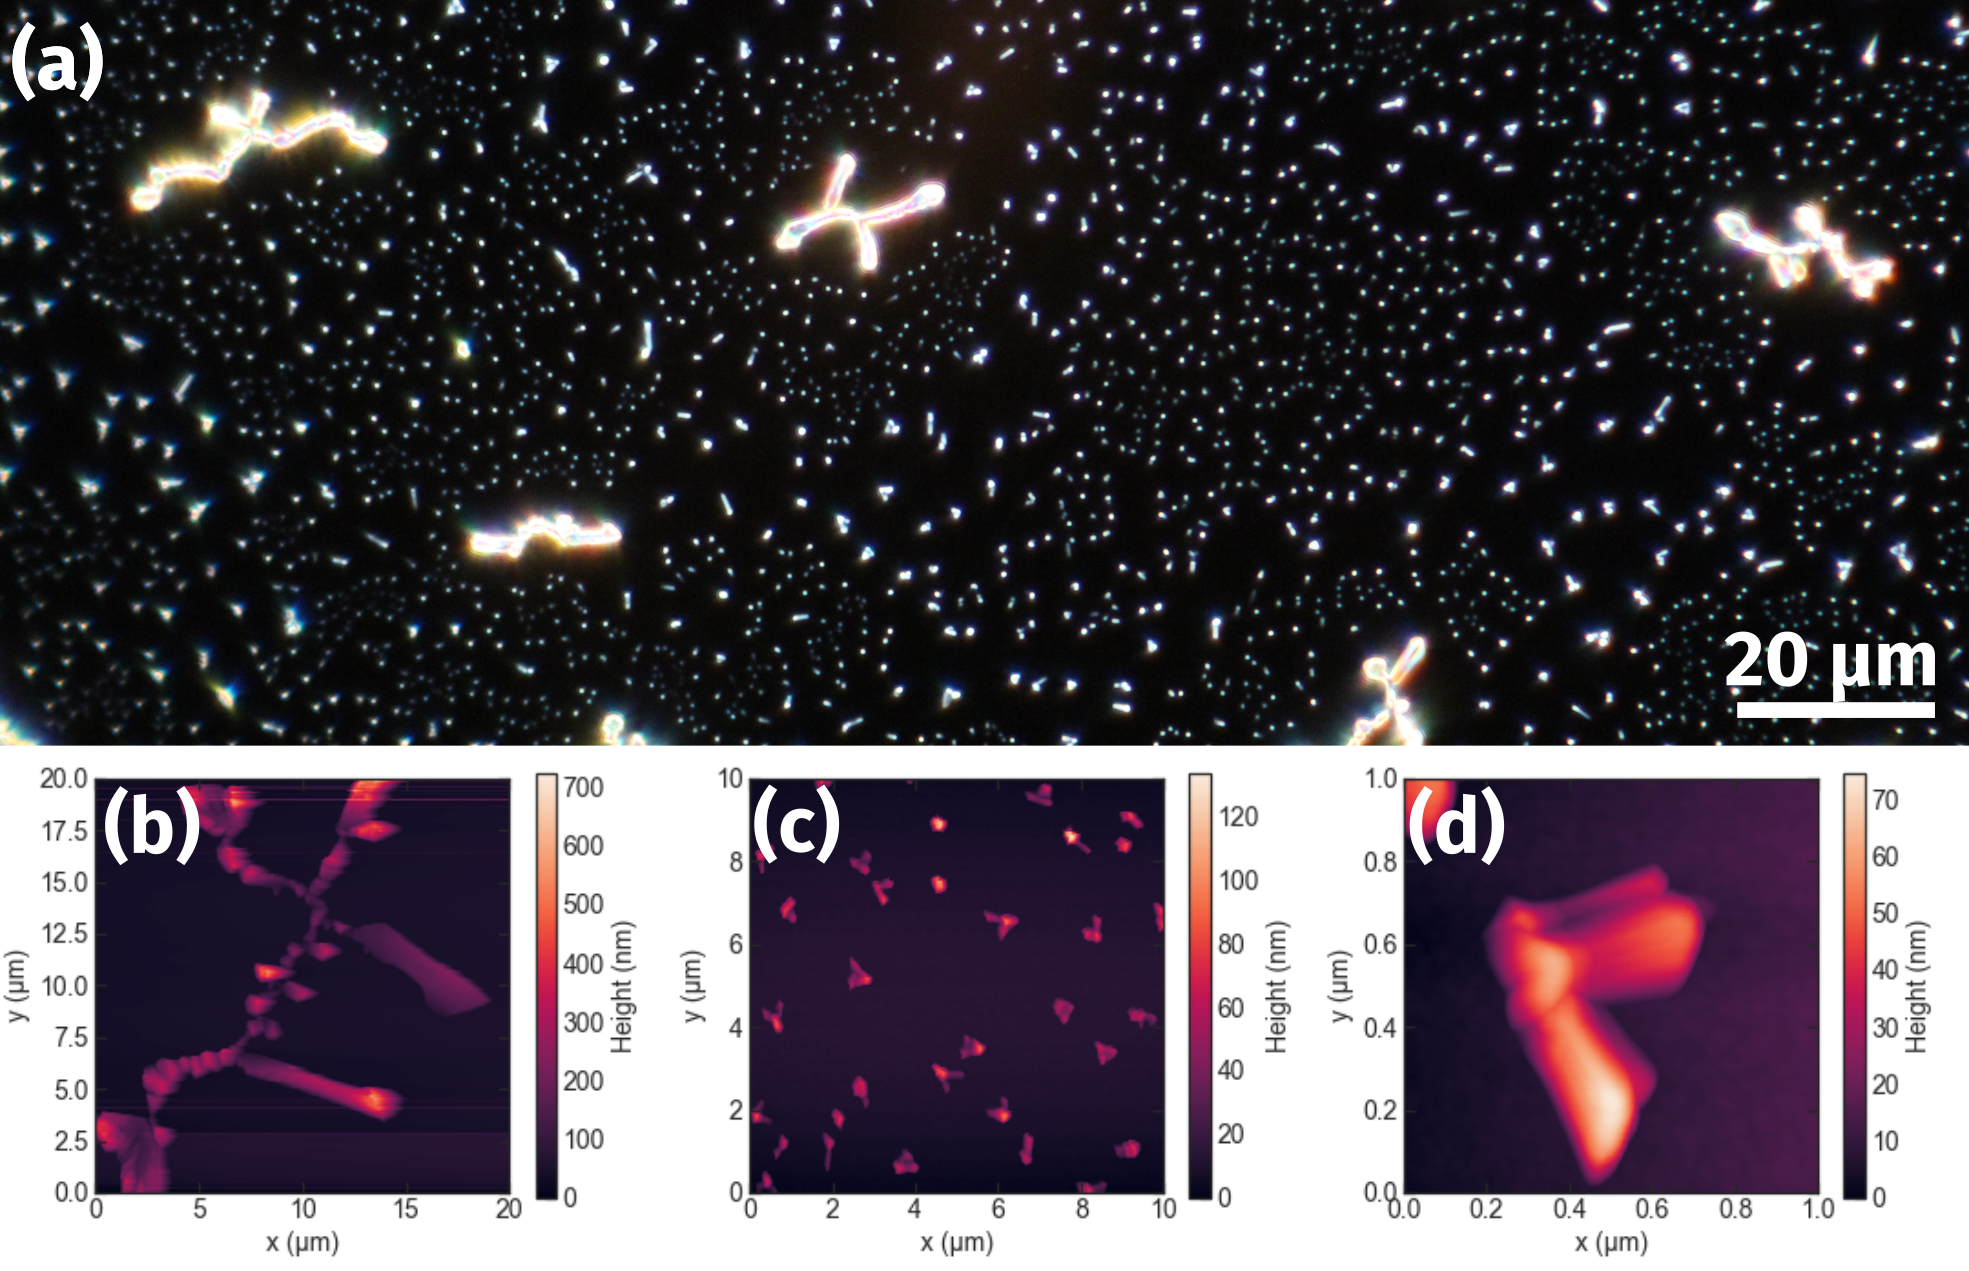
\includegraphics[]{{chapter-experimental-methods/figs-fabrication/MoreDNA.svg}.png}
	\caption{
		\textbf{Chromosome-shaped oxidation of MoRe thin films.}
		\textbf{(a)} Optical image of MoRe film under dark field illumination after two weeks in ambient conditions.
		\textbf{(b-d)} AFM images of several locations and types on the film:
		Small individual crystallites \textbf{(b)} serve as seed islands on the film surface \textbf{(c)}, which then agglomerate into chromosome-shaped strands \textbf{(d)}, covering the entire film surface \textbf{(a)}.
		MoRe film thickness was \SI{100}{\nano\meter}.
	}
	\label{fig:MoreDNA}
\end{figure}

\begin{figure}
	\centering
	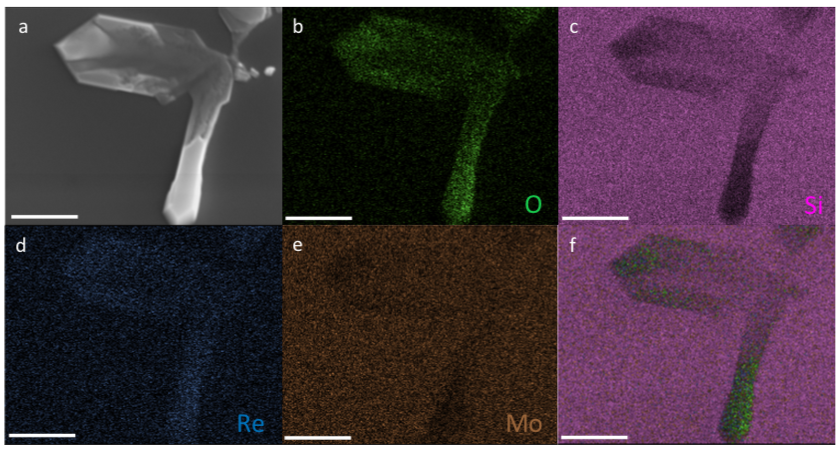
\includegraphics[width=\linewidth]{chapter-experimental-methods/figs-fabrication/pics/MoRe_EDX}
	\caption{
	\textbf{EDX spectra of MoRe crystallites on silicon substrate.}
	\textbf{a,} SEM image of a region in the MoRe layer.
	\textbf{b-e,} EDX elemental maps of O, Si, Re and Mo respectively.
	\textbf{f,} Superposition of the \textbf{b-e} elemental maps.
	All scale bars \SI{2}{\micro\meter}.
	Courtesy of Dr. Miguel Tinoco-Rivas/Conesa-Boj lab, TU Delft.
	}
	\label{fig:moreedx}
\end{figure}